\begin{frame}
    \frametitle{Visualizzare ed Elaborare documenti XML}
    \addtocounter{nframe}{1}
    
    %\begin{center}
    %    
\includegraphics[width=.2\textwidth]{../imgs/tei-r.pdf}
    %\end{center}
    %\textit{In parte già disponibili nei moduli TEI di base}

     \begin{block}{Documenti Object Model (DOM)}
        The Document Object Model (DOM) is a language-independed application programming interface (API) for accessing and manipulating XML documents (e HTML).
        \\ The DOM maps out an entire XML document as a hierarchy of nodes.

    %     \emph{Per la critica testuale indispensabili i moduli}
        %  \begin{itemize}
        %     \item Controllare la codifica e correggere i refusi
        %     \item Assicurarsi che tutto sia stato trascritto correttamente
        %     \item Mostrare il testo a persone che non conoscono XML-TEI
        %     \item Disporre di una versione del lavoro fruibile
        % \end{itemize}
     \end{block}

\end{frame}


\begin{frame}
    \frametitle{Visualizzare ed Elaborare documenti XML}
    \addtocounter{nframe}{1}
    
    \begin{center}
        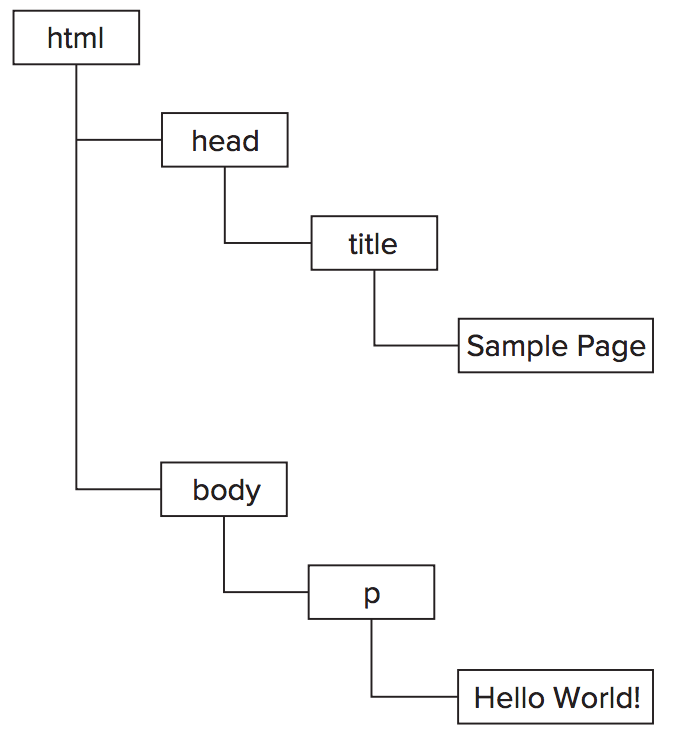
\includegraphics[width=.7\textwidth]{imgs/XML-DOM.png}
    \end{center}
    \textit{In parte già disponibili nei moduli TEI di base}

\end{frame}

\begin{frame}
    \frametitle{Visualizzare ed Elaborare documenti XML}
    \addtocounter{nframe}{1}
    
    %\begin{center}
    %    
\includegraphics[width=.2\textwidth]{../imgs/tei-r.pdf}
    %\end{center}
    %\textit{In parte già disponibili nei moduli TEI di base}

     \begin{block}{Documenti Object Model (DOM)}
        Each part of an XML-TEI documenti is a type of a node containing different kinds of data

     \end{block}

     \begin{block}{Documenti Object Model (DOM)}
        Grazie alla rappresentazione gerarchica messa a disposizione dal DOM è possibile avere un livello di controllo a granularità molto fine per manipolare quasi tutti gli aspetti del documento.
     \end{block}
     
\end{frame}

\begin{frame}
    \frametitle{Visualizzare ed Elaborare documenti XML}
    \addtocounter{nframe}{1}
    
    %\begin{center}
    %    
\includegraphics[width=.2\textwidth]{../imgs/tei-r.pdf}
    %\end{center}
    %\textit{In parte già disponibili nei moduli TEI di base}

     \begin{block}{Documenti Object Model (DOM): espressività}
        Nodes can be removed, added, replaced, and modified easily by using the DOM API.
     \end{block}

     \begin{block}{Documenti Object Model (DOM)}
        Il modello DOM è una specifica e una raccomandazione del consorzio di standardiziazione Web W3C.
        \\\url{URL/TO/DOM/W3C/RECOMMENDATION}
     \end{block}
     
\end{frame}

\begin{frame}
    \frametitle{Visualizzare ed Elaborare documenti XML}
    \addtocounter{nframe}{1}
    
    %\begin{center}
    %    
\includegraphics[width=.2\textwidth]{../imgs/tei-r.pdf}
    %\end{center}
    %\textit{In parte già disponibili nei moduli TEI di base}

     \begin{block}{Documenti Object Model (DOM): Browser-Indipendent}
        Una importante caratteristica del Modello e delle API DOM è la sua indipendenza dalla tecnologia di implementazione.
        
     \end{block}

     \begin{block}{Tecnologia indipendente dal software}
        DOM dovrebbe essere cross-platform, ma in realtà non tutti i browser implementano allo stesso modo le specifiche, così come non tutti i browser sono allineati all'ultima versione delle funzionalità (copertura non al 100\%).
       
     \end{block}
     
\end{frame}


\begin{frame}
    \frametitle{Visualizzare ed Elaborare documenti XML}
    \addtocounter{nframe}{1}
    
    %\begin{center}
    %    
\includegraphics[width=.2\textwidth]{../imgs/tei-r.pdf}
    %\end{center}
    %\textit{In parte già disponibili nei moduli TEI di base}

     \begin{block}{DOM Levels}
       Esistono diverse versioni (livelli) dello standard DOM nonché diverse sezioni all'interno di esso.
     \end{block}

     \begin{block}{DOM Levels}
       Per implementare nel modo più efficace possibile il Modello DOM, questo consta di 5 diverse versioni o approcci, detti livelli, a loro volta suddivisi in moduli.
     \end{block}
     
\end{frame}

\begin{frame}
    \frametitle{Visualizzare ed Elaborare documenti XML}
    \addtocounter{nframe}{1}
    
    %\begin{center}
    %    
\includegraphics[width=.2\textwidth]{../imgs/tei-r.pdf}
    %\end{center}
    %\textit{In parte già disponibili nei moduli TEI di base}

     \begin{block}{le API con il linguaggio di programmazione javascript}
       E' possibile sfruttare usando javascript nativo la rappresentazione ad albero di un documento XML e le funzionalità che DOM mette a disposizione per accedere, manipolare ed estrarre informazioni da un documento XML.
     \end{block}
     
\end{frame}


\begin{frame}
    \frametitle{Visualizzare ed Elaborare documenti XML}
    \addtocounter{nframe}{1}
    
    %\begin{center}
    %    
\includegraphics[width=.2\textwidth]{../imgs/tei-r.pdf}
    %\end{center}
    %\textit{In parte già disponibili nei moduli TEI di base}

     \begin{block}{DOM Level 0}
       Il livello 0 del DOM indica la madalità di operare fuori dalle specifiche W3C.
     \end{block}
     

     \begin{block}{DOM Level 0}
        Con DOM Level 0 si suppongono anche scelte imiplementative non cross-platform e non browser-independent.
      \end{block}

\end{frame}

\begin{frame}
    \frametitle{Visualizzare ed Elaborare documenti XML}
    \addtocounter{nframe}{1}
    
    %\begin{center}
    %    
\includegraphics[width=.2\textwidth]{../imgs/tei-r.pdf}
    %\end{center}
    %\textit{In parte già disponibili nei moduli TEI di base}

     \begin{block}{DOM Level 1}
       DOM Level 1 è la prima versione dello standard (raccomandazione W3C nel 1998). La specifica definisce  oggetti, proprietà e funzionalità di base per navigare e manipolare la struttura di un documento XML (e HTML).
     \end{block}
     

     \begin{block}{DOM Level 1}
        Il DOM Level 1 è diviso in due sezioni:
        \begin{itemize}
            \item[1] \textbf{Generica} per la gestione di documenti XML e HTML
            \item[2] \textbf{Specifica} per documenti HTML che estende la prima.
        \end{itemize}
      \end{block}

\end{frame}

\begin{frame}
    \frametitle{Visualizzare ed Elaborare documenti XML}
    \addtocounter{nframe}{1}
    
    %\begin{center}
    %    
\includegraphics[width=.2\textwidth]{../imgs/tei-r.pdf}
    %\end{center}
    %\textit{In parte già disponibili nei moduli TEI di base}

     \begin{block}{DOM Level 2}
       \textit{DOM Level 2} è un estensione del livello 1 e aggiunge a quest'ultimo numerose funzionalità e specifiche sezioni, come la gestione degli eventi e dei fogli di stile CSS.
     \end{block}
     

     \begin{block}{DOM Level 2}
       Tra i vari moduli che \textit{DOM Level 2} aggiunge, di particolare interesse è il modulo \textbf{DOM Traversal and Range}
      \end{block}

\end{frame}

\begin{frame}
    \frametitle{Visualizzare ed Elaborare documenti XML}
    \addtocounter{nframe}{1}
    
    %\begin{center}
    %    
\includegraphics[width=.2\textwidth]{../imgs/tei-r.pdf}
    %\end{center}
    %\textit{In parte già disponibili nei moduli TEI di base}

     
      Lo standard \textit{DOM Level 3} ha raggiunto lo status di raccomandazione W3C nel 2004.
     

     \begin{block}{DOM Level 3}
        \begin{itemize}
            \item Migliora ed estende il modulo di gestione degli eventi definito nel DOM Level 2
            \item Aggiunge funzionalità per supportare tutta la specifica della versione 1.0 di XML (es.: \textbf{XML namespace}, \textbf{XPath}, \textbf{DOM Validaton})
            \item Caricamento e salvataggio dei documenti con serializzazione XML (\textbf{DOM Load and Save}).
        \end{itemize}
       
      \end{block}

\end{frame}


\begin{frame}
    \frametitle{Visualizzare ed Elaborare documenti XML}
    \addtocounter{nframe}{1}
    
    %\begin{center}
    %    
\includegraphics[width=.2\textwidth]{../imgs/tei-r.pdf}
    %\end{center}
    %\textit{In parte già disponibili nei moduli TEI di base}

     \begin{block}{DOM Level 4}
     \textit{DOM Level 4} è la prossima versione ed estensione del Modello DOM sulla quale sta lavorando il W3C. Ancora non ha raggiunto lo status di raccomandazione e non è ancora supportata dai browser. 
     \end{block}
     

     \begin{block}{DOM Level 4}
       
        \textbf{TROVARE QUALCHE NUOVA FREATURE E IL RAPPORTO CON ECMASCRIPT O ALTRO}
       
      \end{block}

\end{frame}

\begin{frame}
    \frametitle{Visualizzare ed Elaborare documenti XML}
    \addtocounter{nframe}{1}
    
    %\begin{center}
    %    
\includegraphics[width=.2\textwidth]{../imgs/tei-r.pdf}
    %\end{center}
    %\textit{In parte già disponibili nei moduli TEI di base}

     \begin{block}{Supporto dei browser alle specifiche DOM}
        DOM support became a huge priority for most browser vendors, and efforts have been ongoing to improve support with each release.
     \end{block}
     
\end{frame}


\begin{frame}
    \frametitle{Visualizzare ed Elaborare documenti XML}
    \addtocounter{nframe}{1}
    
    %\begin{center}
    %    
\includegraphics[width=.2\textwidth]{../imgs/tei-r.pdf}
    %\end{center}
    %\textit{In parte già disponibili nei moduli TEI di base}

     \begin{block}{Supporto dei browser alle specifiche DOM}
        
     \end{block}
     
\end{frame}


